\documentclass{sintefbeamer}

\usepackage[french]{babel}
\usepackage[T1]{fontenc}
\usepackage{lmodern}
% packages, font, color, and newcommands
\usepackage{amsfonts, amsmath, oldgerm, lmodern, bm}
% \usepackage[font={footnotesize}]{caption}
\usepackage{natbib}
\usepackage{url}
\usepackage{tikz}
\usepackage{amssymb}
\usepackage{amsmath}
\usepackage{amsthm}
\usepackage{mathrsfs}
\usepackage{empheq}
\usepackage{mdframed}
\usepackage{bm}
\usepackage{animate}
\usepackage{xcolor,colortbl}
\usepackage{graphicx}
\usepackage{pgfplots}
\bibliographystyle{apalike}
\usefonttheme{serif}
\usetikzlibrary{calc}
% \title{Theoretical prediction of the Reynolds stress in low inertial buoyant emulsion.}
\title{Curiculum vitae.}
\logo{}
\author{\underline{Nicolas Fintzi}}
% \date{Created on May 22, 2022}
\setbeamertemplate{title page}{%
  \vskip0pt plus 1filll%
  \hspace{-12mm}% Pull back the box in an inelegant way - but it works!
  \begin{beamercolorbox}[wd=0.57
    \textwidth,sep=10pt,leftskip=8mm]{title}%
    % {
\includegraphics[width = 0.15\textwidth]{image/Logo_IFPEN.png}}
    % {
\includegraphics[width = 0.15\textwidth]{image/Sorbonne.jpg}}
    \vspace{60pt}
    
    {\usebeamerfont{title}\inserttitle}
    
    {\usebeamerfont{subtitle}\insertsubtitle}
    
    {\usebeamerfont{author}\usebeamercolor[fg]{author}\insertauthor}
    
    {\usebeamerfont{date}\usebeamercolor[fg]{date}\insertdate}
    \thispagestyle{empty}
  \end{beamercolorbox}

  % {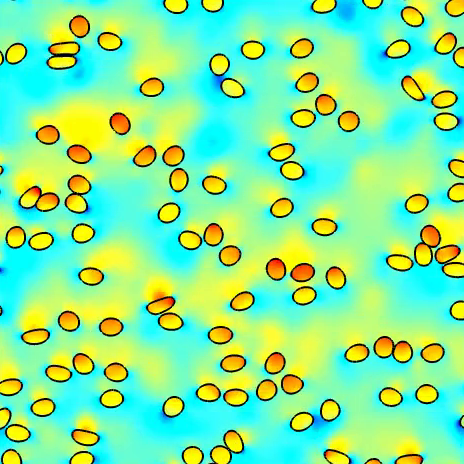
\includegraphics[width =0.3 \textwidth]{image/pic/bulles.png}}
}

% \titlebackground{image/800good.png}

% document body
\addtobeamertemplate{navigation symbols}{}{%
    \usebeamerfont{footline}%
    \usebeamercolor[fg]{footline}%
    % \hspace{1em}%
    % \vspace{1em}%
    \insertframenumber/\inserttotalframenumber
}
\usepackage{stmaryrd}

\usepackage{amsmath}


\begin{document}

\maketitle
\begin{frame}{Avant la th\`ese \ldots}
  \textbf{Formation :}
  \begin{enumerate}
      \item $2016$ - $2018$ : DUT G\'enie M\'ecanique et Productique (GMP) Lyon 1.
      \item $2018$ - $2019$ : INSA Lyon : Sp\'ecialit\'e G\'enie M\'ecanique (Lyon).
      \item $2019$ - $2021$ : INSA Lyon : Sp\'ecialit\'e Plasturgie et composite (Oyonnax).
    \end{enumerate}
\end{frame}

  
  
  


\begin{frame}[fragile]
  \frametitle{Stage de M2 dans le d\'epartement R15 \`a l'IFPEN.}
  
  \begin{minipage}[c]{0.6\textwidth}
    \textbf{Motivation - Ebullated, fluidized \\ and fixed beds of cylindrical particles}
  \begin{figure}
    \centering
    \begin{tikzpicture}
      \node (pic1) at (0,0) {\includegraphics[width = 0.4\textwidth]{/work/fintzin/CYLINDERS_PROJECT/RoadToJFM/image/LITBOUILLONANT.png}};
      \draw[red,very thick] (0,0) circle(0.75);
      \node (pic2) at (4,0) {\includegraphics[height=0.4\textwidth]{/work/fintzin/CYLINDERS_PROJECT/RoadToJFM/image/TRIperio/triperiodiquePIC.png}};
      \draw[red, very thick,->](0.75,0)--(pic2.west)node[midway,below]{Zoom};
      % \node[very thick] at (pic1.south){\textbf{Macroscale}};
      % \node[very thick] at (pic2.south){\textbf{Microscale}};
      \draw[black!50!blue,->,very thick](-0.2\textwidth,-1)--(-0.2\textwidth,0.6)node[midway,left]{$\Delta P$};
      \draw[black!50!blue,->,very thick](pic2)++(0.11\textwidth,-0.2\textwidth)--++(0,0.4\textwidth)node[midway,right]{$\frac{\partial P }{\partial x}$};
      % \draw[very thick,]
    \end{tikzpicture}
    % 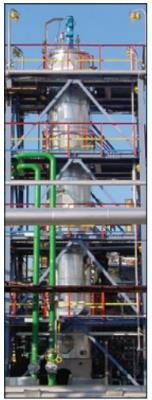
\includegraphics[width = 0.4\textwidth]{image/process.jpg}

  \end{figure}

  \end{minipage}\hfill
\begin{minipage}[c]{0.4\textwidth}
  \textbf{Highly complex coupled physical phenomena}:
  \begin{itemize}
    \item 2 or 3 phases: fluid, gas, and solid
    \item Species transport
    \item Chemical reaction
    \item Heat and mass transfer
  \end{itemize}
  \textbf{Parameters}:
  \begin{itemize}
    \item $1 < Re_p < 200$
    \item $\phi \approx 0.3$
    \item $\chi \approx 6$
   \end{itemize}
  \end{minipage}
  \textbf{Objectives} $\rightarrow$ \underline{Estimate $\Delta P$ for any set of parameters}

\end{frame}

\begin{frame}
  \frametitle{Premi\`eres \'etape : Modelisation d'une particle cyldrique isol\'e avec le code de calcul \texttt{OpenFoam} }
  
  \begin{columns}
    \begin{column}{0.5\textwidth}
  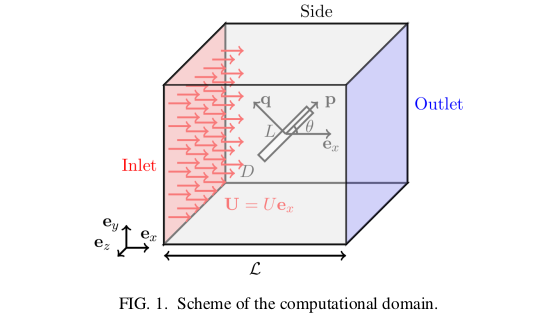
\includegraphics[width=\textwidth]{image/cylindre_trans.png}

      
    \end{column}
    \begin{column}{0.5\textwidth}
      \textbf{Force : }
      \begin{equation*}
        \textbf{f} = 
        \mu L (\textbf{R}^{Re}+ \mathbf{S}^{Re})\cdot\textbf{u}
      \end{equation*}
      \textbf{Moment angulaire : }
      \begin{equation*}
        \textbf{t} = 
        \mu L^2 \textbf{T}^\text{Re}\cdot \textbf{u}
      \end{equation*}
    \end{column}
  \end{columns}
\pause 
\centering
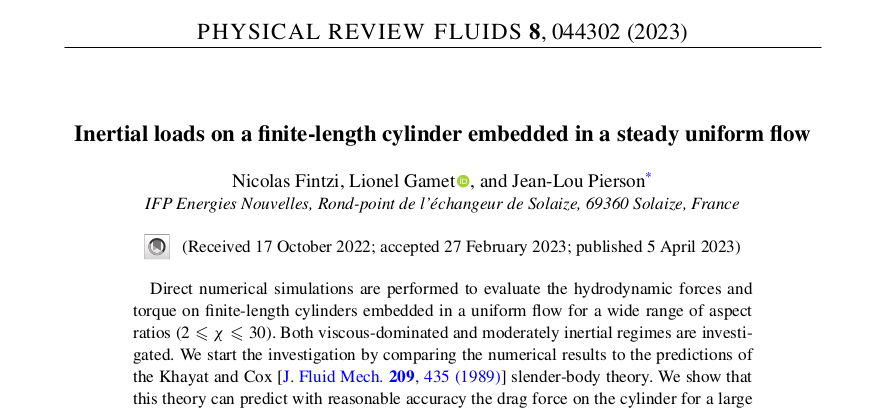
\includegraphics[width=0.5\textwidth]{image/paper.png}

\end{frame}
\begin{frame}
  \frametitle{Deux\`eme \'etape : Modelisation d'un lit fixe de particules cylindrique (\texttt{OpenFoam}).}

  \centering
\includegraphics[width=0.9\textwidth]{/work/fintzin/CYLINDERS_PROJECT/RoadToJFM/image/cbeau.png}

% $\to$ Projet repris part Jelena Marack (R12) 
\begin{itemize}
  \item Mise en place d'un code pour la simulaiton de volume représentatif de lit fixe de particules cylindrique. 
\end{itemize}
\end{frame}
\begin{frame}
  \frametitle{Deux\`eme \'etape : Modelisation d'un lit fixe de particules cylindrique (\texttt{OpenFoam}).}

  \centering
% \includegraphics[width=0.5\textwidth]{/work/fintzin/CYLINDERS_PROJECT/RoadToJFM/image/cbeau.png}
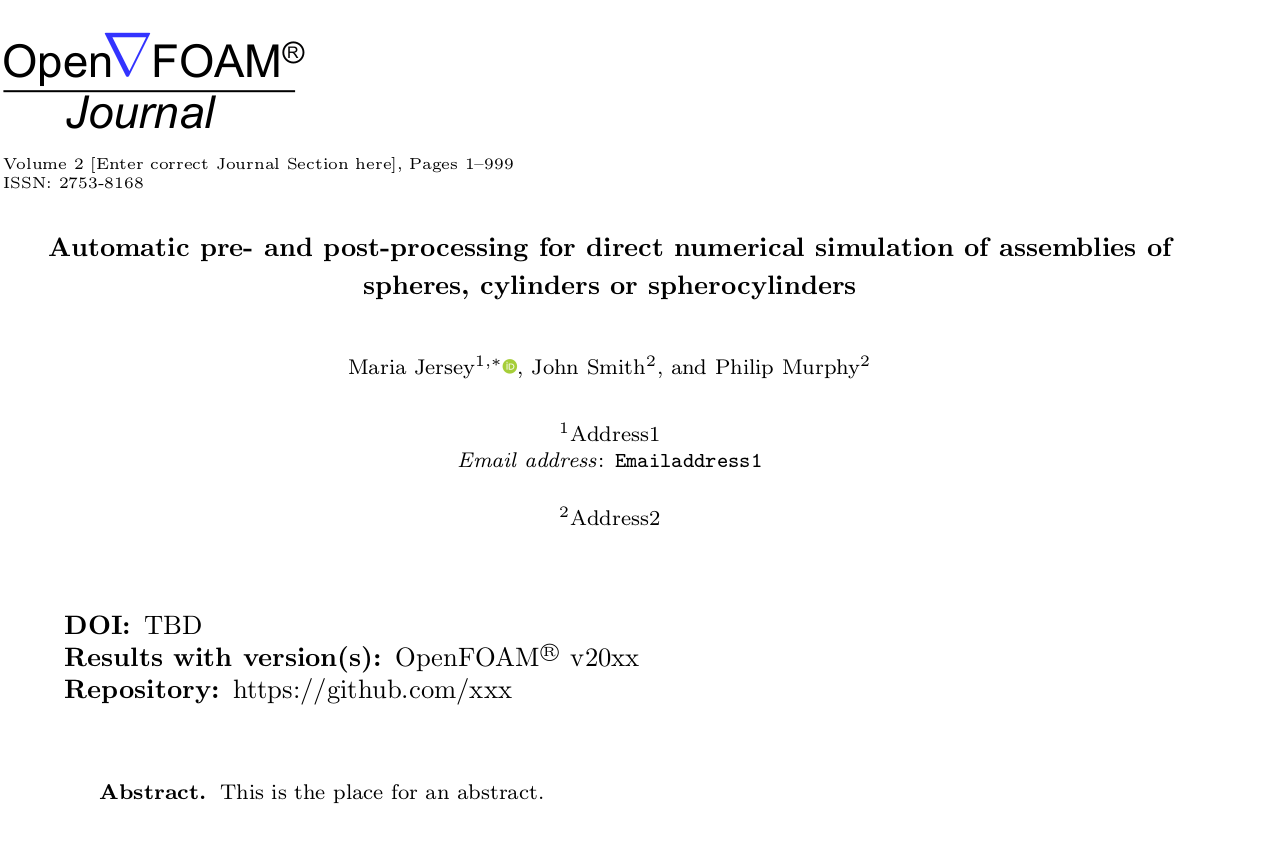
\includegraphics[width=0.6\textwidth]{image/OpenfoamJ.png}

$\to$ Projet repris part Jelena Marack (Post-Doc R12) 
\end{frame}


\begin{frame}
  \frametitle{Ma th\`ese}

  

\end{frame}
\end{document}

